\begin{enumerate}[label=\thesection.\arabic*.,ref=\thesection.\theenumi]
\numberwithin{equation}{enumi}

\item
Find the Phase Margin of $G(s)$ in degrees where
\begin{align}
G(s) = \frac{2}{(s+1)(s+2)}
\end{align}
\solution \textbf{Phase Margin}:It is the difference between phase of the system and $-180^{\circ}$ at the gain crossover frequency,(the gain crossover frequency being the frequency at which the open-loop gain first reaches 1).\\
Phase Margin is given by,
\begin{align}
P.M=\phi-\angle G(j\omega)|_{\omega=\omega_{pc}}=\phi+180^{\circ}
\end{align}
where,
\begin{align}
\phi=\angle G(j\omega)|_{\omega=\omega_{gc}}
\label{eq:1}
\end{align}
$\omega_{pc}$ is the Phase crossover frequency (The frequency at which the phase of open-loop transfer function reaches -180$^{\circ}$).\\
$\omega_{gc}$ is the Gain crossover frequency (The frequency at which the gain of the open-loop transfer fuction reaches 1).\\
Given,

\begin{align}
G(s) = \frac{2}{(s+1)(s+2)} 
\\
G(j\omega)=\frac{1}{(j\omega+1)(j\omega+2)} 
\end{align}
We can find magnitude and phase as

\begin{align}
|G(j\omega)|=\frac{2}{(\sqrt{\omega^2+1})(\sqrt{\omega^2+4})}
\\
\angle G(j\omega)=- tan^{-1}(\omega) - tan^{-1}(\frac{\omega}{2}) \label{eq:2}
\end{align}

We know that,
Gain in dB = 0 at $\omega=\omega_{gc}$
\begin{align}
20log_{10}|G(j\omega_{gc})|=0 
\\
|G(j\omega_{gc})|=1
\\
\frac{2}{(\sqrt{\omega_{gc}^2+1})(\sqrt{\omega_{gc}^2+4})}=1
\end{align}
Solving we get,
\begin{align}
\omega^2_{gc}(\omega^2_{gc}+5)=0
\\
=> \omega_{gc}=0,+j\sqrt{5},-j\sqrt{5}
\end{align}
As frequency is a real quantity
\\Hence, $\omega_{gc} \neq$ Imaginary
\begin{align}
\therefore  \omega_{gc} =0
\end{align}
From (\ref{eq:1}) and (\ref{eq:2})
\begin{align}
\phi= \angle G(j\omega_{gc})= -tan^{-1}(\omega_{gc})-tan^{-1}(\frac{\omega_{gc}}{2})
\end{align}

\begin{align}
=> \phi=0^{\circ}
\\
\therefore P.M=180^{\circ}+0^{\circ}=180^{\circ}
\end{align}

\item
We can verify the above result using phase plot.The following code plots Fig(\ref{fig:ee18btech11017})
\begin{lstlisting}
codes/ee18btech11017.py
\end{lstlisting}
\item
The Phase plot is as shown,
\begin{figure}[!h]
  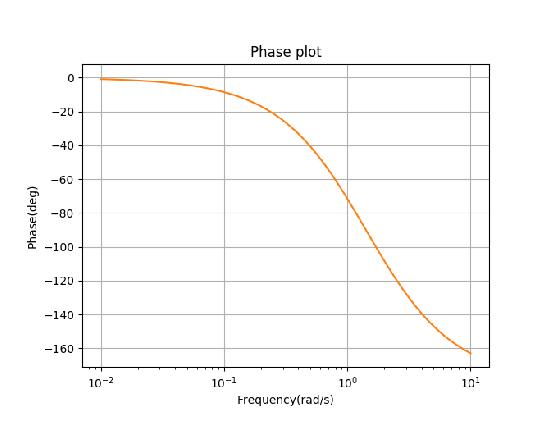
\includegraphics[width=\columnwidth]{./figures/ee18btech11017.eps}
  \caption{}
  \label{fig:ee18btech11017}
\end{figure}
We can observe that at $\omega_{gc}=0$ , $\phi=0^{\circ}$
\\
\begin{align}
\therefore P.M=180^{\circ}
\end{align}
\item
\textbf{Application:} 
Phase margin is measure of stability in closed-loop, dynamic-control systems.(i.e, For stability of a system both gain margin and phase margin should be positive.)
\item
\textbf{Example:}Phase Margin is a measure of stability. \\
Consider a unity negative feedback system with open loop gain ,
\\
\begin{align}
G(s)=\frac{10000}{s(s+10)^{2}}
\label{eq:3} 
\end{align}
We can find mgnitude and phase as \\
\begin{align}
|G(j\omega)|=\frac{10^{4}}{\omega \sqrt{(\omega^{2}+10^{2})^{2}}} \\
\angle G(j\omega)=-90^{\circ}-2tan^{-1}\frac{\omega}{10} \label{eq:5} 
\end{align}
At the gain cross over frequency $\omega_{gc}$,$|G(j\omega)|=1$
\\
\begin{align}
\frac{10^{4}}{\omega_{gc} \sqrt{(\omega_{gc}^{2}+10^{2})^{2}}}=1 \\
\end{align}
Simplifying we get,
\begin{align}
\omega_{gc}^{3}+10^{2}\omega_{gc}-10^{4}=0 \\
=> \omega_{gc}=20,-10+20j,-10-20j
\end{align}
As frequency is a real quantity
\\Hence, $\omega_{gc} \neq$ Imaginary
\begin{align}
\therefore  \omega_{gc} =20   \label{eq:6} 
\end{align}
From (\ref{eq:5}) and (\ref{eq:6}) we get,
\begin{align}
P.M=180^{\circ}-90^{\circ}-2tan^{-1}(\frac{\omega_{gc}}{10}) \\
=> P.M=-36.9^{\circ}
\end{align}
We can verify the above result using phase plot.The following code plots Fig(\ref{fig:ee18btech11017_1})
\begin{lstlisting}
codes/ee18btech11017.py
\end{lstlisting}
The Phase plot is as shown,
\begin{figure}[!h]
  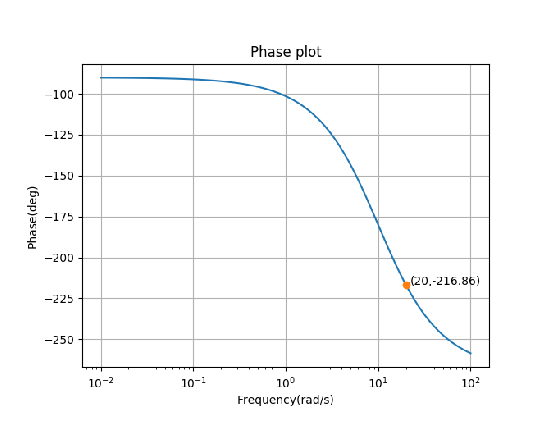
\includegraphics[width=\columnwidth]{./figures/ee18btech11017_1.eps}
  \caption{}
  \label{fig:ee18btech11017_1}
\end{figure}
We can observe that at $\omega_{gc}=20$ , $\phi=-216.86^{\circ}$
\\
\begin{align}
\therefore P.M=180^{\circ}+-216.86^{\circ}=-36.9^{\circ} \\
\end{align}
As Phase Margin is negative . Therefore the closed loop system is unstable .
We can verify closed loop stability using Routh-Hurwitz criterion.


\item
Verifying the above example using Routh-Hurwitz criterion.\\
Let $T(s)$ be Closed loop transfer function ,
\begin{align}
T(s)=\frac{N(s)}{D(s)}=\frac{G(s)}{1+G(s)}
\end{align}
The characteristic equation is 
\begin{align}
D(s)=0  \\
1+G(s)=0 
\end{align}

\begin{align}
=> s^{3}+20s^{2}+100s+10000=0   \label{eq:7} 
\end{align}
\\
Constructing routh array for (\ref{eq:7})..,
\begin{align}
\mydet{s^3\\s^2\\s}
\mydet{1 & 100 & 0 \\ 20 & 10000 & 0 \\ -400 & 0 & 0}
\end{align}\\

\begin{align}
\mydet{s^3\\s^2\\s\\s^0}
\mydet{1 & 100 & 0 \\ 20 & 10000 & 0 \\ -400 & 0 & 0 \\ 10000 & 0 & 0}
\end{align}\\

There are two sign changes in the first column of the routh array. So, two poles lie on right half of s-plane. \\
Therefore,the system is unstable.\\
The following code generates routh array.
\begin{lstlisting}
codes/RouthHurwitz.py
\end{lstlisting}


\item
Now consider $G(s)$ from (\ref{eq:3}),in above example and multiply it with $H(s)=10^{-1}$. So, now open loop gain becomes $G(s)H(s)$.
\begin{align}
G(s)H(s)=\frac{1000}{s(s+10)^{2}}
\label{eq:8} 
\end{align}

We can find mgnitude and phase as \\
\begin{align}
|G(j\omega)H(j\omega)|=\frac{10^{3}}{\omega \sqrt{(\omega^{2}+10^{2})^{2}}} \\
\angle G(j\omega)H(j\omega)=-90^{\circ}-2tan^{-1}\frac{\omega}{10} \label{eq:9} 
\end{align}

At the gain cross over frequency $\omega_{gc}$,$|G(j\omega)H(j\omega)|=1$
\\
\begin{align}
\frac{10^{3}}{\omega_{gc} \sqrt{(\omega_{gc}^{2}+10^{2})^{2}}}=1 \\
\end{align}

Simplifying we get,
\begin{align}
\omega_{gc}^{3}+10^{2}\omega_{gc}-10^{3}=0 \\
=> \omega_{gc}=6.82,-3.41+11.6j,-3.41-11.6j
\end{align}
As frequency is a real quantity
\\Hence, $\omega_{gc} \neq$ Imaginary
\begin{align}
\therefore  \omega_{gc} =6.82   \label{eq:10} 
\end{align}

From (\ref{eq:9}) and (\ref{eq:10}) we get,
\begin{align}
P.M=180^{\circ}-90^{\circ}-2tan^{-1}(\frac{\omega_{gc}}{10}) \\
=> P.M=21.42^{\circ}
\end{align}

We can verify the above result using phase plot.The following code plots Fig(\ref{fig:ee18btech11017_2})
\begin{lstlisting}
codes/ee18btech11017.py
\end{lstlisting}
The Phase plot is as shown,
\begin{figure}[!h]
  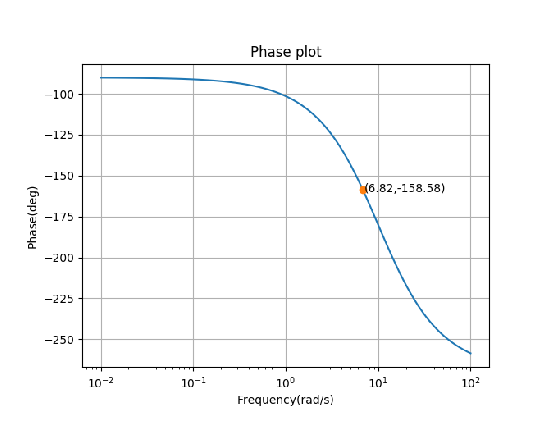
\includegraphics[width=\columnwidth]{./figures/ee18btech11017_2.eps}
  \caption{}
  \label{fig:ee18btech11017_2}
\end{figure}

We can observe that at $\omega_{gc}=6.82$ , $\phi=-158.58^{\circ}$
\\
\begin{align}
\therefore P.M=180^{\circ}+-158.58^{\circ}=21.42^{\circ} \\
\end{align}
As Phase Margin is positive. Therefore the closed loop system is stable .
We can verify closed loop stability using Routh-Hurwitz criterion.

\textbf{Verification}: \\

Verifying the above example using Routh-Hurwitz criterion.\\
Let $T(s)$ be Closed loop transfer function ,
\begin{align}
T(s)=\frac{N(s)}{D(s)}=\frac{G(s)H(s)}{1+H(s)G(s)}
\end{align}
The characteristic equation is 
\begin{align}
D(s)=0  \\
1+G(s)H(s)=0 
\end{align}

\begin{align}
=> s^{3}+20s^{2}+100s+1000=0   \label{eq:11} 
\end{align}
\\
Constructing routh array for (\ref{eq:11})..,
\begin{align}
\mydet{s^3\\s^2\\s}
\mydet{1 & 100 & 0 \\ 20 & 1000 & 0 \\ 50 & 0 & 0}
\end{align}\\

\begin{align}
\mydet{s^3\\s^2\\s\\s^0}
\mydet{1 & 100 & 0 \\ 20 & 1000 & 0 \\ 50 & 0 & 0 \\ 1000 & 0 & 0}
\end{align}\\

There are no sign changes in the first column of the routh array. So, all the poles lie on left half of s-plane. \\
Therefore,the system is stable.\\
The following code generates routh array.
\begin{lstlisting}
codes/RouthHurwitz.py
\end{lstlisting}








\end{enumerate}
